% xelatex

\documentclass[a4paper,10pt]{article}

\usepackage{marvosym}
\usepackage{fontspec}                               % for loading fonts
\usepackage{xunicode,xltxtra,url,parskip}           % other packages for formatting
\RequirePackage{color,graphicx}
\usepackage[usenames,dvipsnames]{xcolor}
\usepackage{fullpage}                               % alternative to layaureo
%\usepackage[big]{layaureo}                         % better formatting of the A4 page
%\usepackage{fullpage}                              % standard margines
%\usepackage{supertabular}                          % for Grades
\usepackage{titlesec}                               % custom \section
\usepackage[none]{hyphenat}                         % disable any hyphenation
\usepackage{graphicx}                               % photo import
\usepackage{wrapfig}                                % image/text wrapping
\usepackage{hyperref}                               % setup hyperref package, and colours for links
\usepackage{setspace}                               % setup line spacing
\usepackage{array}                                  % table lines
\usepackage{ulem}                                   % underlining: for big correct underline distance

\setlength{\parskip}{\baselineskip}

\definecolor{linkcolor}{RGB}{10, 40, 155}
\definecolor{mygray}{gray}{0.25}
\definecolor{linegray}{gray}{0.6}
\definecolor{darkgreen}{RGB}{54, 138, 83}

\def\name{Pesho Ivanov}
\def\myline{\color{linegray}\vline}
\def\interestsSpace{\\[1.3mm]}                          % wider line spacing

\newcommand{\minorcolor}[1]{\textcolor{mygray}{#1}}
\newcommand{\wide}{\addfontfeature{LetterSpace=3.0}}    % wide letter spacing
\newcommand{\comment}[1]{\small\textcolor{darkgreen}{\,\,//\,#1}}
\newcommand{\mydate}[1]{\minorcolor{\textsc{#1}}}
\newcommand{\bracketcomment}[1]{{\small\textit{\minorcolor{(#1)}}}}
\newcommand{\mysect}[2]{\vbox{\section{#1}{#2}}}

\hypersetup{
  colorlinks = true,
  urlcolor = linkcolor,
  pdfauthor = {\name},
  pdfkeywords = {Computer Science},
  pdftitle = {\name: Curriculum Vitae},
  pdfsubject = {Curriculum Vitae},
  pdfpagemode = UseNone
}

%FONTS
\defaultfontfeatures{Mapping=tex-text}
\setmainfont[SmallCapsFont = Fontin SmallCaps]{Fontin}

%CV Sections
\titleformat{\section}{\Large\scshape\raggedright}{}{0em}{}[\color{linegray}\titlerule]  % section style
\titlespacing{\section}{0pt}{15pt}{0pt}

% MARGINES
\addtolength{\oddsidemargin}{-3mm}
\addtolength{\evensidemargin}{-3mm}
\addtolength{\textwidth}{8mm}

\addtolength{\topmargin}{0mm}
\addtolength{\textheight}{25mm}

\linespread{1.15}                               % line spacing

%--------------------BEGIN DOCUMENT----------------------
\begin{document}
\pagestyle{empty}                               % non-numbered pages
\font\fb=''[cmr10]''                            % for use with \LaTeX command

% *** Photo ***
% \begin{wrapfigure}{r}{4.5cm}
%         \setlength\fboxsep{0pt}
%         \setlength\fboxrule{0.1pt}
%         \vspace{-50pt}\fbox{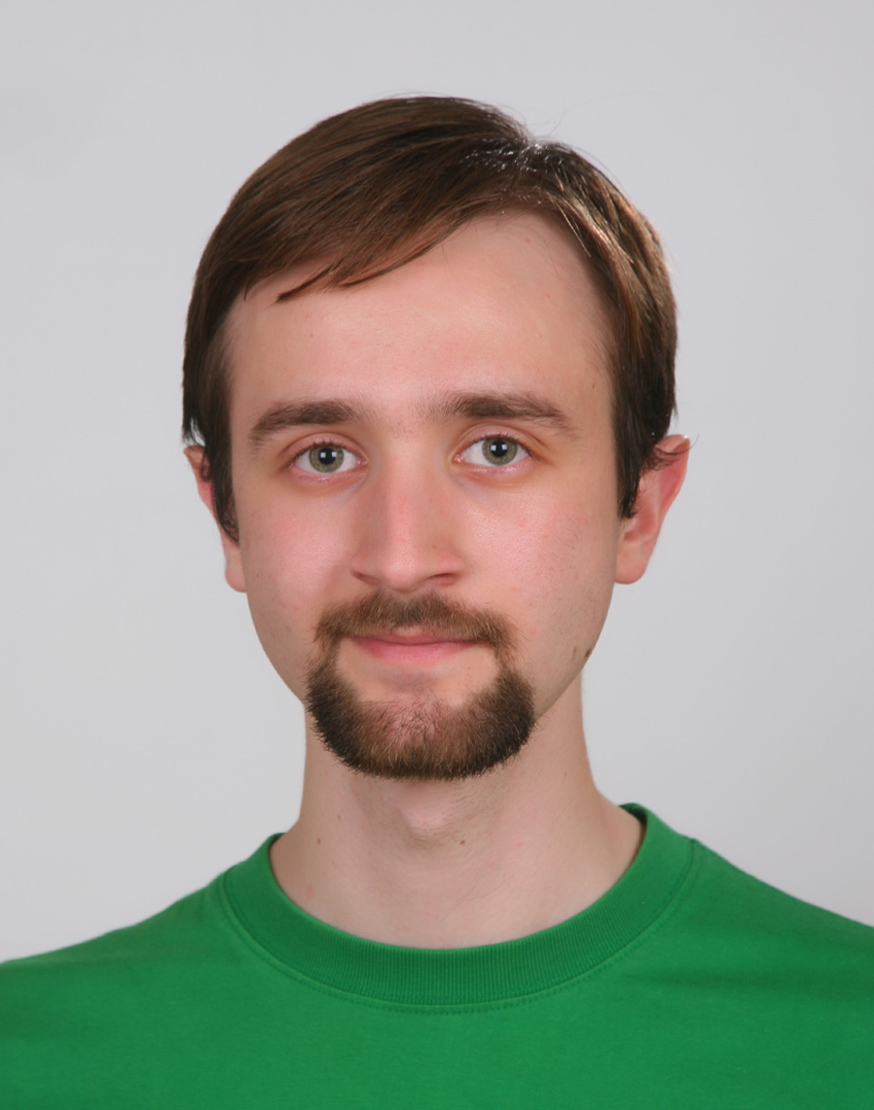
\includegraphics[width=33mm]{PetarIvanov2013.jpg}}
% \end{wrapfigure}

\begin{wrapfigure}{r}{5cm}
          \vspace{-35pt}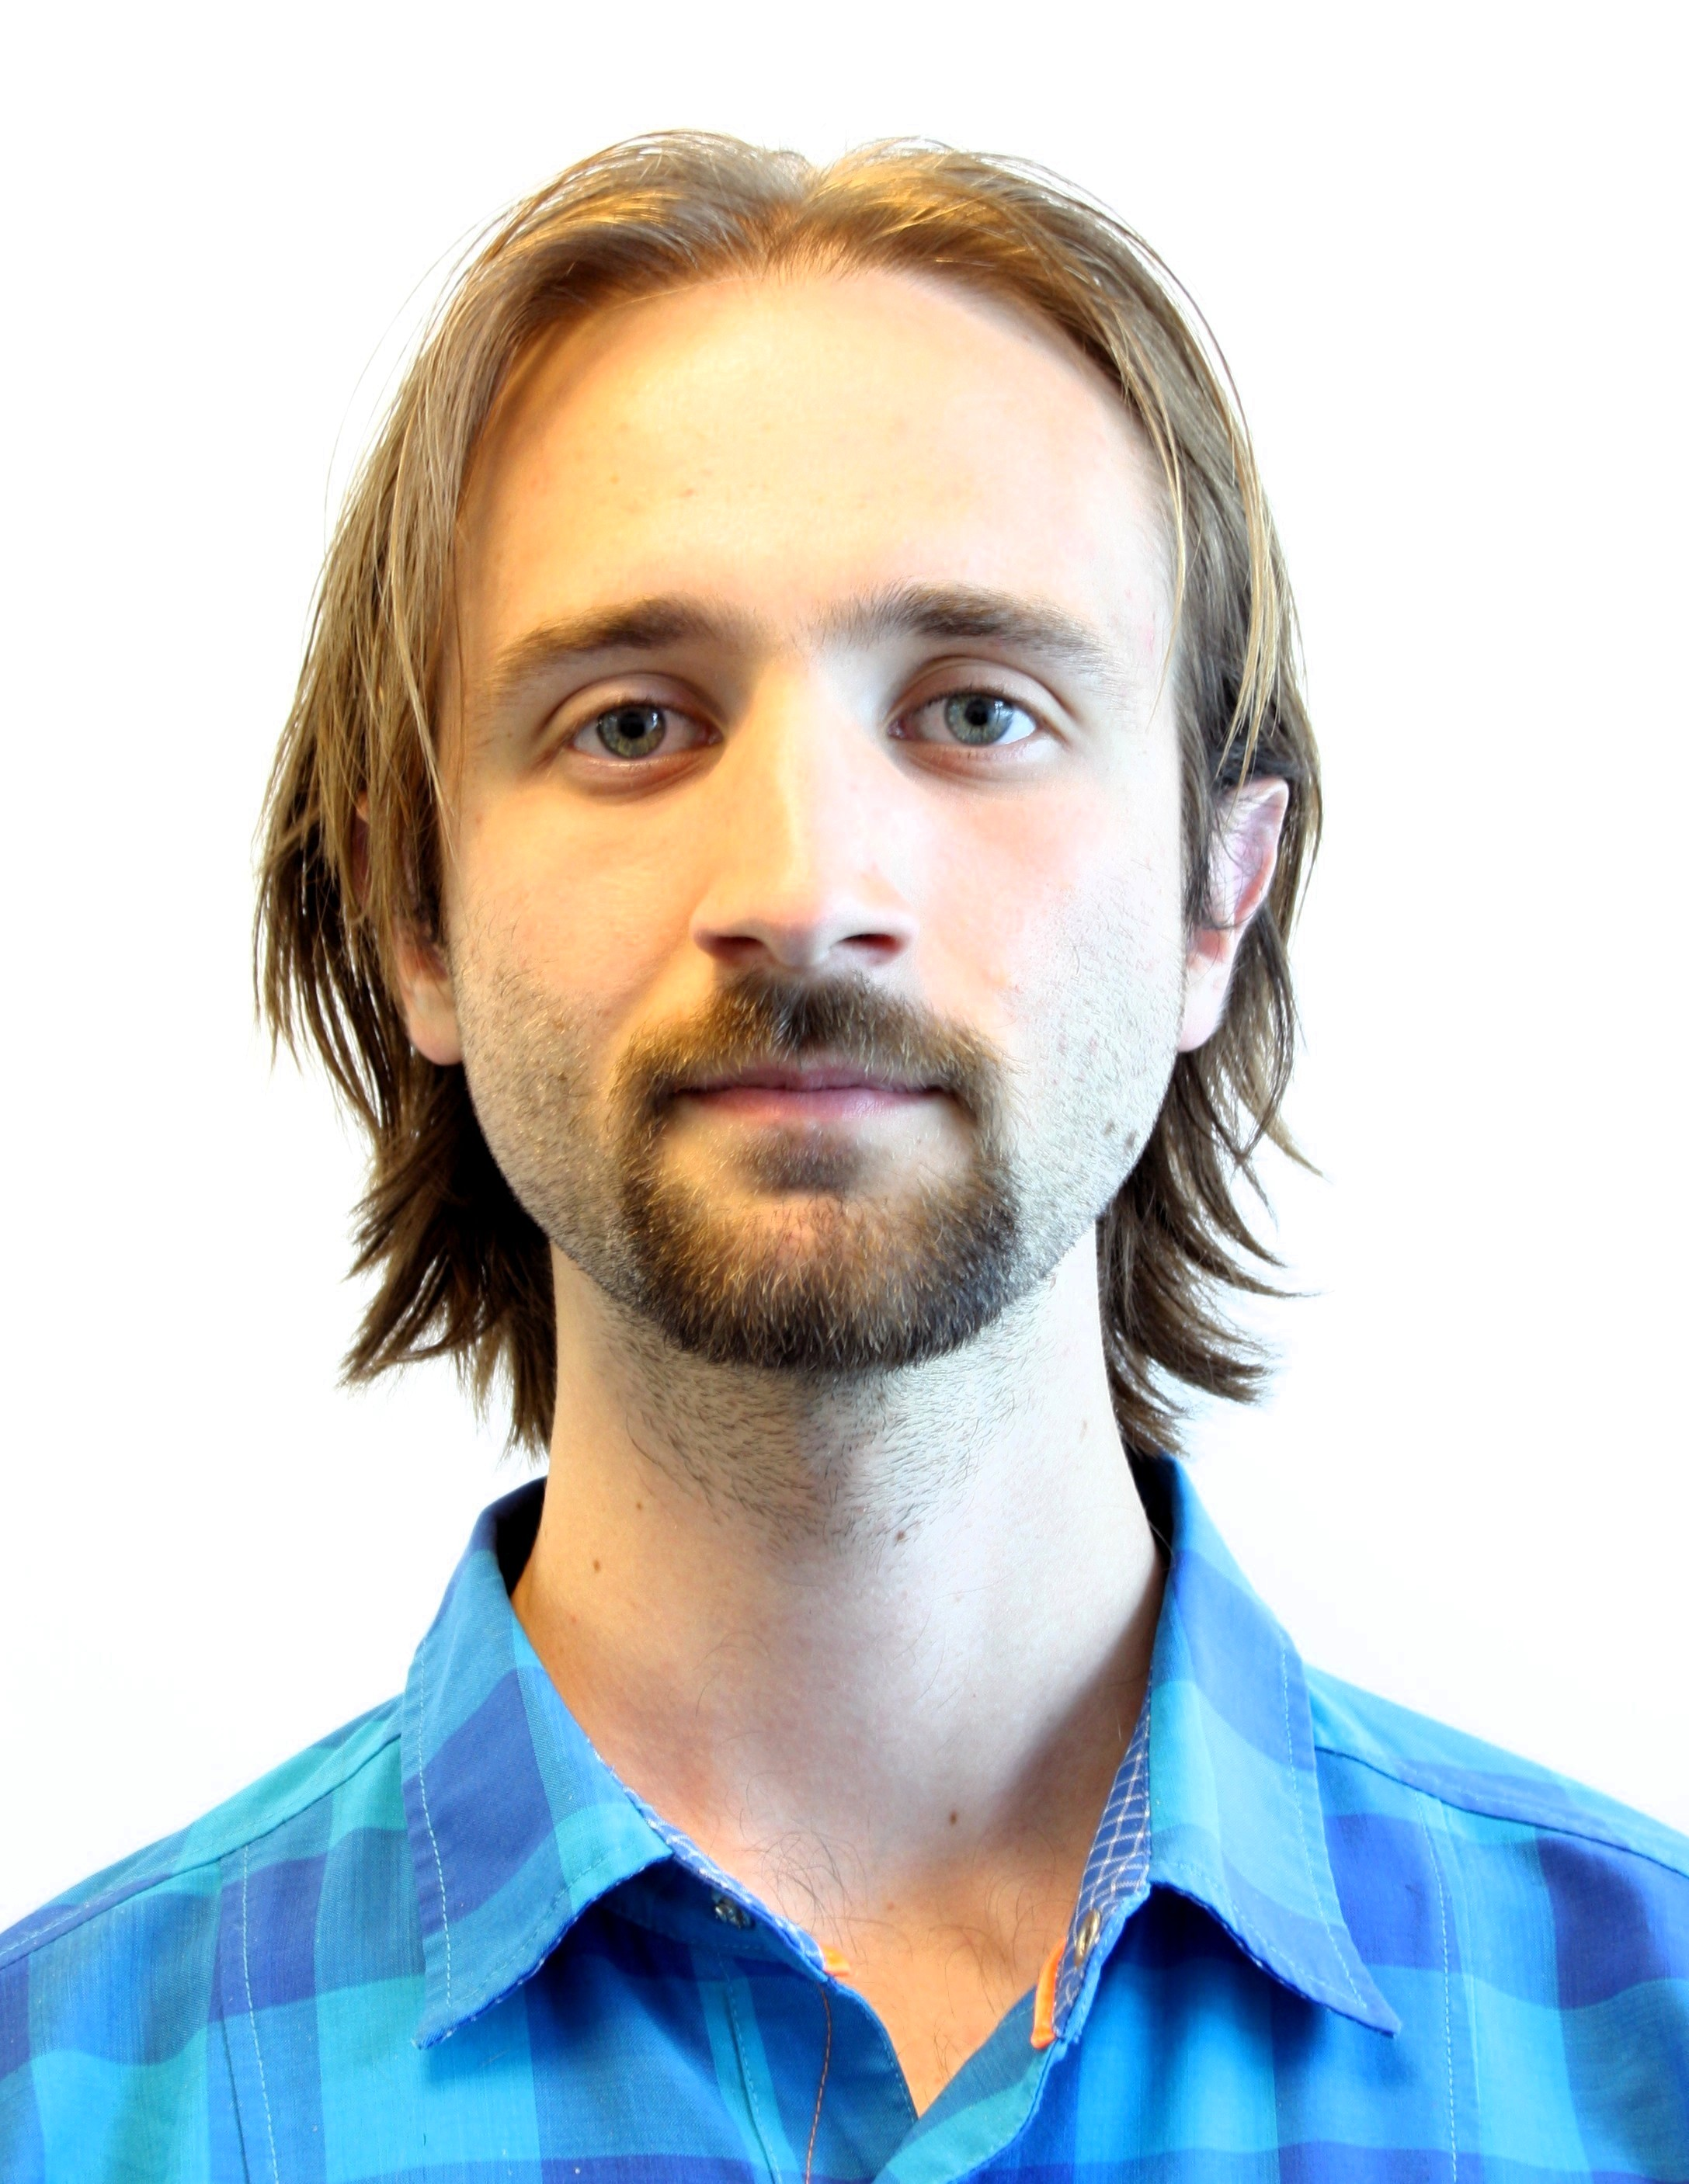
\includegraphics[width=35mm]{PetarIvanov2015.jpg}
\end{wrapfigure}

% *** Profile ***
\par{\raggedright\Huge\textbf{\vspace{-3mm}\hspace{0mm}\name}}\\        % big name on the top
\vspace{-5mm}{\color{linegray}\rule{10.5cm}{0.1mm}}\\

\hspace{4mm}\begin{tabular}{rl}
        \minorcolor{passport:} & \textsc{Petar Ivanov}\\
        \minorcolor{born:} & \textsc{29 May 1989} in Shumen, Bulgaria\\
        %\minorcolor{address:} & Manessestrasse \textsc{64}, Zurich \textsc{8003}, Switzerland\\
        \minorcolor{email:} & \href{mailto:ivanov@pesho.info}{ivanov@pesho.info}\\
        \minorcolor{url:} & \href{https://www.sri.inf.ethz.ch/people/pesho}{sri.inf.ethz.ch/people/pesho}\\
        \minorcolor{github:} & \href{https://github.com/pesho-ivanov/}{github.com/pesho-ivanov}\\
\end{tabular}
\bigskip


% Section: *** Summary ***
\mysect{Summary}{
%\begin{center}
%\vspace{1mm}
  \begin{tabular}{c}
      PhD student at ETH Zurich with strong background in Computational Biology,\\
      Algorithms and Data structures. Worked as a Software engineer at Google.\\
      Loves learning and teaching and enjoys informatics competitions. In a hurry to do good.\\
    \end{tabular}
%\end{center}
}  % end of Summary


% Section: *** Education ***
\mysect{Education}{
%\vspace{2mm}
\begin{tabular}{r!{\myline}p{14cm}}
        \mydate{Apr 2017 --- now}      &   PhD student on \textbf{Reliable Computational Biology}\\
                                            &   \textit{Prof. Martin Vechev's} Secure, Reliable, and Intelligent Systems Lab (SRI)\\
                                            &   Computer Science department\\
                                            &   ETH Zurich, Switzerland\\


        \multicolumn{2}{c}{}\\
        \mydate{Apr 2015 --- Feb 2017}      &   Master degree in \textbf{Software Engineering} \bracketcomment{extra-mural} \\
                                            &   Thesis: \textit{Framework for Genomic Reconstruction Algorithms}\\
                                            &   Shumen University, Bulgaria\\


        \multicolumn{2}{c}{}\\
        \mydate{Jun 2014}                   &   Bachelor degree in \textbf{Computer Informatics}\\
                                            &   Shumen University, Bulgaria\\
                                            &   \small\textcolor{darkgreen}{\,\,$\uparrow$\,transferred because of a crazy ban from entering Russia}\\
        \mydate{Sep 2009 --- Jun 2013}      &   Specialist degree \bracketcomment{equivalent to Bachelor+Master} in \textbf{Applied Mathematics and Informatics}\\
        \bracketcomment{interrupted by visa issues}
                                            &   Moscow State University, Russia \comment{calculus, Computer vision}\\
                                            %&  Major in Computer vision at \textsc{Graphics \& Media laboratory}\\
                                            %&  \textbf{Faculty of Computational Mathematics and Cybernetics}\\
  %\textbf{Faculty of Mathematics and Informatics}


%        \multicolumn{2}{c}{}\\
%        \mydate{Sep 2011 --- Jun 2013}      &   Master degree \bracketcomment{not accredited} in \textbf{Bioinformatics}
%                                                \comment{+ taught algorithms to biologists}\\
%                                            &   Yandex School of Data Mining, Moscow, Russia\\

        \multicolumn{2}{c}{}\\
        \mydate{Sep 2008 --- Jun 2009}      &   Bachelor degree in \textbf{Computer science}
                                                \comment{+ led seminars in advanced algorithmics}\\
        \bracketcomment{left to Moscow} &  Sofia University, Bulgaria \comment{mainly discrete maths}\\
                                                %\textbf{Faculty of Mathematics and Informatics},
        %{\small\textit{after the first year)}}

       \multicolumn{2}{c}{}\\
        \mydate{Sep 2000 --- Jun 2008}      &   Mathematics and Physics profile
                                                \comment{award for most scientific achievements of his year}\\
                                            &   Shumen High school of Sciences, Bulgaria\\
%\small\textit{
\end{tabular}
}  % end of Education
\par\smallskip

%\hspace{7mm}\textit{\minorcolor{\underline{Core courses passed:}}}
%
%\hspace{1.5mm}\begin{tabular}{r!{\myline}p{5cm}r!{\myline}p{6cm}}
%     \minorcolor{Technical}  &  \textsc{Image Processing} & & \\
%       \minorcolor{courses}  &  \textsc{Video Processing} & & \\
%              & \textsc{Computer Vision}\\
%              & \textsc{Combinatorial Optimization}\\
%              & \textsc{Bioinformatics Tools}\\
%              & \textsc{Computational Geometry}\\
%              & \textsc{Computational Linguistics}\\
%\end{tabular}
%
%\hspace{1.5mm}\begin{tabular}{r!{\myline}p{7cm}}
%  \minorcolor{Biological}  &  \textsc{Algorithms in Bioinformatics} {\small\textit{(x2)}}\\
%  \minorcolor{courses}  &  \textsc{Molecular Biology} {\small\textit{(x2)}}\\
%                            &  \textsc{Microevolution}\\
%                            &  \textsc{Macroevolution}\\
%                            &  \textsc{Immunology}\\
%                            &  \textsc{Embryology}\\
%\end{tabular}

\hspace{7mm}{\textit{\minorcolor{\underline{Additional:}}}

\vspace{-2mm}\hspace{0mm}\begin{tabular}{r!{\myline}p{14cm}}
        \mydate{Sep 2011 --- Jun 2013}      &   Master degree \bracketcomment{not accredited} in \textbf{Bioinformatics}
                                                \comment{+ taught algorithms to biologists}\\
                                            &   \hspace{5mm} Yandex School of Data Mining, Moscow, Russia\\
        \mydate{Jan 2011}       &   \textsc{Vision and Machine-learning Research School}, ENS Lyon, France\\
        \mydate{Jul 2008}       &   \textsc{Russian Summer Informatics Camp}, Kostroma, Russia
                                            \comment{3 weeks of problems and theory}\\
        \mydate{Aug 2007}       &   \textsc{Physics Camp}, Panitsite, Bulgaria
                                            \comment{3 weeks of maths and physics}\\
        \mydate{2004 --- 2007}  &   \textsc{Summer Research Informatics Camp}, Varna, Bulgaria
                                            \comment{2-week problem solving}\\
        \mydate{2001 --- 2008}  &   \textsc{Mathematics and Informatics Private School ``A\&B''}, Shumen, Bulgaria\\
\end{tabular}


\newpage


% Section: *** Internships ***
\mysect{Internships}{
%\vspace{2mm}
\begin{tabular}{r!{\myline}p{14cm}}
        % \multicolumn{2}{c}{}\\
        \mydate{Jun 2016 ---}       &   Bioinformatics internship on Single-cell transcriptomics lymphoma patients\\
        \mydate{Mar 2017}           &   \textit{Prof. Martin Vechev, \href{http://www.srl.inf.ethz.ch/}{Software Reliability Lab}, ETH Zurich}\\
                                    &   \textit{PD Dr. Emmanuella Guenova, \href{http://www.dermatologie.usz.ch/forschung/Seiten/forschungsgruppen.aspx}{Dermatology Clinic}, University of Zurich}\\

        \multicolumn{2}{c}{}\\
        \mydate{Jul 2013 ---}       &   Summer internship on \href{http://bioinf.spbau.ru/spades}{SPAdes} open source genome assembler
                                        \comment{\href{http://pesho.info/wp-content/uploads/chimeras-final.pdf}{chimeras presentation}}\\
        \mydate{Aug 2013}           &   \comment{proof of concept: replication bugs to enhance assembly in open source assembler}\\
                                    &   \textit{Prof. Pavel Pevzner's, \href{http://bioinf.spbau.ru/}{\textbf{Algorithmic Biology Lab}}, St. Petersburg Academic University}\\

        \multicolumn{2}{c}{}\\
        \mydate{Sep 2012 ---}       &   Microbiological models designer
                                        \comment{\href{https://docs.google.com/document/d/1tNkXLaWY3ooA4MEnrbrL2_DOpOaiTlLoFblwzKFZdy0/edit?usp=sharing}{Microcin modelling}}\\
        \mydate{Jun 2013}           &   \textit{Prof. Konstantin Severinov's lab, \href{http://www.genebiology.ru/}{Institute of Gene biology}, Russian Academy of Sciences}\\

        \multicolumn{2}{c}{}\\
        \mydate{Jul 2012 ---}       &   Research internship on probabilistic verification of biological models\\
        \mydate{Aug 2012}           &   \comment{insisted on my own topic on virus-bacteria interaction \href{https://docs.google.com/document/d/1tNkXLaWY3ooA4MEnrbrL2_DOpOaiTlLoFblwzKFZdy0/edit?usp=sharing}{[Summary]}}\\
                                    &   \textit{Prof. Martin Vechev's, \href{http://www.srl.inf.ethz.ch/}{Software Reliability Lab}, ETH Zurich}\\

        \multicolumn{2}{c}{}\\
        \mydate{Jul 2011 ---}       &   Computational Geometry Algorithms Library (\href{http://www.cgal.org/}{CGAL}) internship\\
        \mydate{Aug 2011}           &   \href{http://code.google.com/soc/}{Google Summer of Code}
                                        \comment{implemented topological operators on tetrahedral meshes}\\

        \multicolumn{2}{c}{}\\
        \mydate{Jul 2007 ---}       &   Developer of a bin-packing genetic algorithm for glass cutting optimization\\
        \mydate{Sep 2007}           &   \textit{\href{http://telepol.net/telepol.net/}{Telepol Net}, Bulgaria}
                                        \comment{appreciating evolution and first algorithm in production}\\
\end{tabular}
}  % end of Internships

% http://www.hansenlab.org/cv_bibliography_tex
\mysect{Publications}{
\begin{tabular}{!{\myline}l}
        \textsc{AStarix}: Fast and Optimal Sequence-to-Graph Alignment\\
        \textbf{P. Ivanov}, B. Bichsel, H. Mustafa, A. Kahles, G. Rätsch, M. Vechev\\
        \textit{International Conference on Research in Computational Molecular Biology (RECOMB) 2020}\\

        \multicolumn{1}{c}{}\\
        \textsc{Debin}: Predicting debug information in stripped binaries \\
        J. He, \textbf{P. Ivanov}, P. Tsankov, V. Raychev, M. Vechev\\
        \textit{Proceedings of the 2018 ACM SIGSAC Conference on Computer and Communications Security}\\

        \multicolumn{1}{c}{}\\
        Ineffective antibody-dependent cellular cytotoxicity in patients with cutaneous T cell lymphoma\\
        Y. Chang, M. Ziegler, D. Ignatova, \textbf{P Ivanov}, R. Profanter, K. Kerl, R. Dummer,\\
        \,\,\,\, E. Contassot, L. French, A. Cozzio, S. Misailovic, W. Hoetzenecker, M. Vechev, E. Guenova\\
        \textit{EXPERIMENTAL DERMATOLOGY, 2018}\\

%        \cite{ivanov2020astarix}
%\printbibliography[title=Journal Articles (peer reviewed),keyword=published]

\end{tabular}
}  % end of Publications

%Section: *** Teaching ***
\mysect{Teaching}{
%\vspace{2mm}
\begin{tabular}{r!{\myline}p{14cm}}
        %\multicolumn{2}{c}{}\\
        \mydate{Sep 2017 --- now}   &   Teaching Assistant for the courses\\
                                    &   \hspace{5mm} \textit{Algolab}, \textit{Data structures and Algorithms}, \textit{Parallel programming}, \\
                                    &   \hspace{5mm} \textit{Rigorous Software Engineering}, \textit{Reliable AI},\textit{Theoretical Informatics}\\
%                                        \comment{leading an evolutional computational project}\\
                                    &   Computer Science department, ETH Zurich\\

        \multicolumn{2}{c}{}\\
        \mydate{Sep 2015,}          &   Supervisor of high school students\\
%                                        \comment{leading an evolutional computational project}\\
        \mydate{Sep 2018}           &   \textit{\href{http://www.sciencexplore.org/}{Science\&Arts school ``Science Xplore''}}, Viseu, Portugal\\

        \multicolumn{2}{c}{}\\
        \mydate{Nov 2013 ---}       &   Informatics competitions trainer for high school students\\
%                                        \comment{praparing algorithmic lecture notes}\\
        \mydate{Jun 2014}           &   \textit{\href{http://ab-bg.com/}{Mathematics and Informatics Private School ``A\&B''}}, Shumen, Bulgaria\\

        \multicolumn{2}{c}{}\\
        \mydate{Nov 2013 ---}       &   Teaching Assistant for the \textit{Coursera} \href{https://www.coursera.org/course/bioinformatics}{Bioinformatics course}\\
%                                        \comment{lectures editing, forum explanations}\\
        \mydate{Jan 2014}           &   \textit{Prof. Pavel Pevzner}, University of California, San Diego\\

        \multicolumn{2}{c}{}\\
        \mydate{Aug 2010}           &   Lecturer at school students informatics camp
                                        \comment{strongest Russian competitors}\\
                                    &   \textit{\href{http://lksh.ru/}{Russian Summer Informatics Camp}, Saratov}\\

        \multicolumn{2}{c}{}\\
        \mydate{Mar 2008 ---}       &   Teaching Assistant for ``Design and Analysis of Algorithms'' course\\
%                                        \comment{led seminars to a group of 20 people}\\
        \mydate{Jun 2009}           &   \textit{Faculty of mathematics and informatics, Sofia University}, Bulgaria\\

        \multicolumn{2}{c}{}\\
        \mydate{Sep 2008 ---}       &   Author of the problems in \href{http://konkurs.musala.com/}{Online programming tournament}\\
        \mydate{Jun 2009}           &   \textit{Musala Soft, Bulgaria}
                                        \comment{mainly discrete optimization problems}\\

        \multicolumn{2}{c}{}\\
        \mydate{2008 --- 2009}      &   Author of problems for Bulgarian Tournaments in Informatics\\
                                        % \comment{4 such competitions}\\
        \mydate{2013 --- 2014}      &   Lecturer at National Informatics Camps\\
                                        % \comment{3 such camps}\\
                                    &   \textit{National Committee in Informatics, Bulgarian Ministry of Education}\\
\end{tabular}
}  % end of Teaching

\newpage

% Section: *** Industry ***
\mysect{Industry}{
%\vspace{2mm}
\begin{tabular}{r!{\myline}p{14cm}}
        % \multicolumn{2}{c}{}\\
        \mydate{Sep 2014 ---}       &   Software Engineer at Search $\supset$ Knowledge $\supset$ Infrastructure\\
        \mydate{Jan 2016}           &   \textit{Google Zurich}\\ %\comment{big data and pipelines}\\
\end{tabular}
}  % end of Industry


% Section: *** Awards ***
\mysect{Awards}{
\par{\vspace{-8mm}\hspace{7cm}{\minorcolor{\textit{the competitions are National Bulgarian if nothing else stated}}}}\\

\vspace{-6mm}\hspace{3.5mm}\begin{tabular}{r!{\myline}p{14cm}}
        \textbf{1}\textsuperscript{st} place    &  \textsc{``Minko Balkanski'' Competition in Informatics '08}\\
        \textbf{11}\textsuperscript{th} place   &  \textsc{TopCoder High School Finals, West Lafayette, USA '08}\\
        \textbf{1}\textsuperscript{st} place    &  \textsc{Autumn Tournament in Informatics '07}\\
        \textbf{1}\textsuperscript{st} place    &  \textsc{Student Competition for the Dean's cup of Sofia University '07}\\
        \textbf{2}\textsuperscript{nd} place    &  \textsc{International Young Physicists Tournament \bracketcomment{regional, in team} '06}\\
        \textbf{1}\textsuperscript{st} place    &  \textsc{``Rumen Grozdanov'' Informatics and Mathematics Tournament '06}\\
        \textbf{1}\textsuperscript{st} place    &  \textsc{Winter Tournament in Informatics '06}\\
\end{tabular}
\medskip

\hspace{3mm}\begin{tabular}{@{•\enskip}p{14.5cm}}
% \setlength{\parindent}{1cm}
        Awarded as a \textbf{National Laureate in Informatics}, Bulgaria \textsc{'08}\\
        Scholarship for \textbf{science achievements} of \href{http://www.afbulgaria.org/}{\textsc{American Foundation for Bulgaria}} \textsc{'07}---\textsc{'08}\\
        Participated in the \textbf{final rounds} of the \textsc{Bulgarian Olympiad in Informatics} \textsc{'05}---\textsc{'08}\\
        Participated in the \textbf{final rounds} of the \href{http://community.topcoder.com/tc?module=Static\&d1=tournaments\&d2=home}{\textsc{TopCoder High School}}, West Lafayette, USA \textsc{'07}---\textsc{'08}\\
        Participated in the \textbf{final rounds} of ``\href{http://konkurs.musala.com/}{\textsc{Musala Soft and PC Magazine}}'' competition \textsc{'07}---\textsc{'08}\\
        % Participated in the tournament \textsc{Australian Mathematics Trust}, \textsc{'05}---\textsc{'07}\\
        % Scholarship for \textit{excellent grades}, \textsc{'06}, \textsc{'07} and \textsc{'08}\\
\end{tabular}
}  % end of Awards


% Section: *** Computer Skills ***
\mysect{General skills}{
%\vspace{2mm}
\begin{tabular}{rp{14cm}}
  Algorithms:     &  Graphs, Combinatorics, Strings, Geometry, Optimization, Dynamic Programming\\
  Programming:    &  \textbf{C\,/\,C++ (STL)}, Python (NumPy, SciPy, MatPlotLib), MATLAB\\
  Tools:          &  Unix, Bash, Vim, Git, {\fb \LaTeX}\\ % HTML, CSS,
  Speaks:         &  English, Russian, Bulgarian\\
\end{tabular}
}  % end of Skills


% Section: *** Activities ***
%\section{Activities \,\textbf{:")}}
\mysect{Activities}{
%\vspace{-2mm}
\hspace{2mm}\begin{tabular}{@{•\enskip}ll}
% \setlength{\parindent}{1cm}
        Solving algorithmic problems &
              \comment{\href{http://www.topcoder.com/tc?module=MemberProfile&cr=10205233}{\textsc{TopCoder}}, \href{http://acm.timus.ru/author.aspx?id=30642}{\textsc{Timus}}, \href{http://rosalind.info/users/cheater_no1/}{\textsc{Rosalind}} }\\
        Supporting crowdsourcing, FOSS and open data &
              \\%\comment{\href{https://github.com/pesho-ivanov/}{GitHub profile} }\\
        %Founded a project for describing educational systems &
        %      \comment{\href{http://students-abroad.info/}{students-abroad.info} }\\
        Editing \href{https://en.wikipedia.org/wiki/User:Cheater_no1}{wikipedia} and a \href{http://pesho-ivanov.github.io/}{personal wiki}\\
        {\wide Running and paragliding} %hiking, biking, dancing, paragliding and running}
              & \comment{\textbf{42.195km~in~3:43h}, \href{http://probeg.org/card.php?id=273}{Zelenograd, Russia, Dec 2011} }\\
              \multicolumn{1}{l}{} & \multicolumn{1}{l}{ \comment{\textbf{100km~in~13:19h}, \href{http://www.vitosha100km.bg/2011/}{Vitosha mountain, Bulgaria, 2012} } }\\
        Meditation & \comment{\textsc{Goenka's 10-day meditation retreat}, 2020}\\

    % CouchSerfing, donating blood, travelling
    % Scientifically interested in \textsc{Computer Vision, Computational Geometry, Bioinformatics, Machine Learning, Genetic Algorithms}\interestsSpace
    %Being impressed by Bioinformatics, Synthetic biology, Combinatorial Optimization, Computer Vision, Computational Geometry, Genetics, Machine Learning, Robotics\interestsSpace
    % \href{https://opensnp.org/users/637}{\textsc{genotype}})\interestsSpace
    % including my own \href{http://pesho.info/category/msu}{\textsc{blog}} about Moscow State University\interestsSpace
    % Practising traditional Bulgarian dances and classical ballroom dances.\interestsSpace
\end{tabular}
}  % end of Activities

\end{document}
